% Chapter 3

\chapter{跨分辨率车辆计数数据集}

\section{数据集简介}
跨分辨率车辆计数数据集收集了日本常陆那珂港的 192 张极低分辨率图像和 8 张高分辨率图像,日期范围为 2016 年至 2019 年。其中LR 图像是www.planet.com 下载的,由 PlanetScope 卫星拍摄,地面分辨率为每像素 3m。为了起到监督作用,HR 图像是在根据相应 LR 图像的日期选择的,这些图像是从 WorldView 捕获的,地面分辨率为每像素 30 厘米。 
\begin{figure}[h]
    \centering
    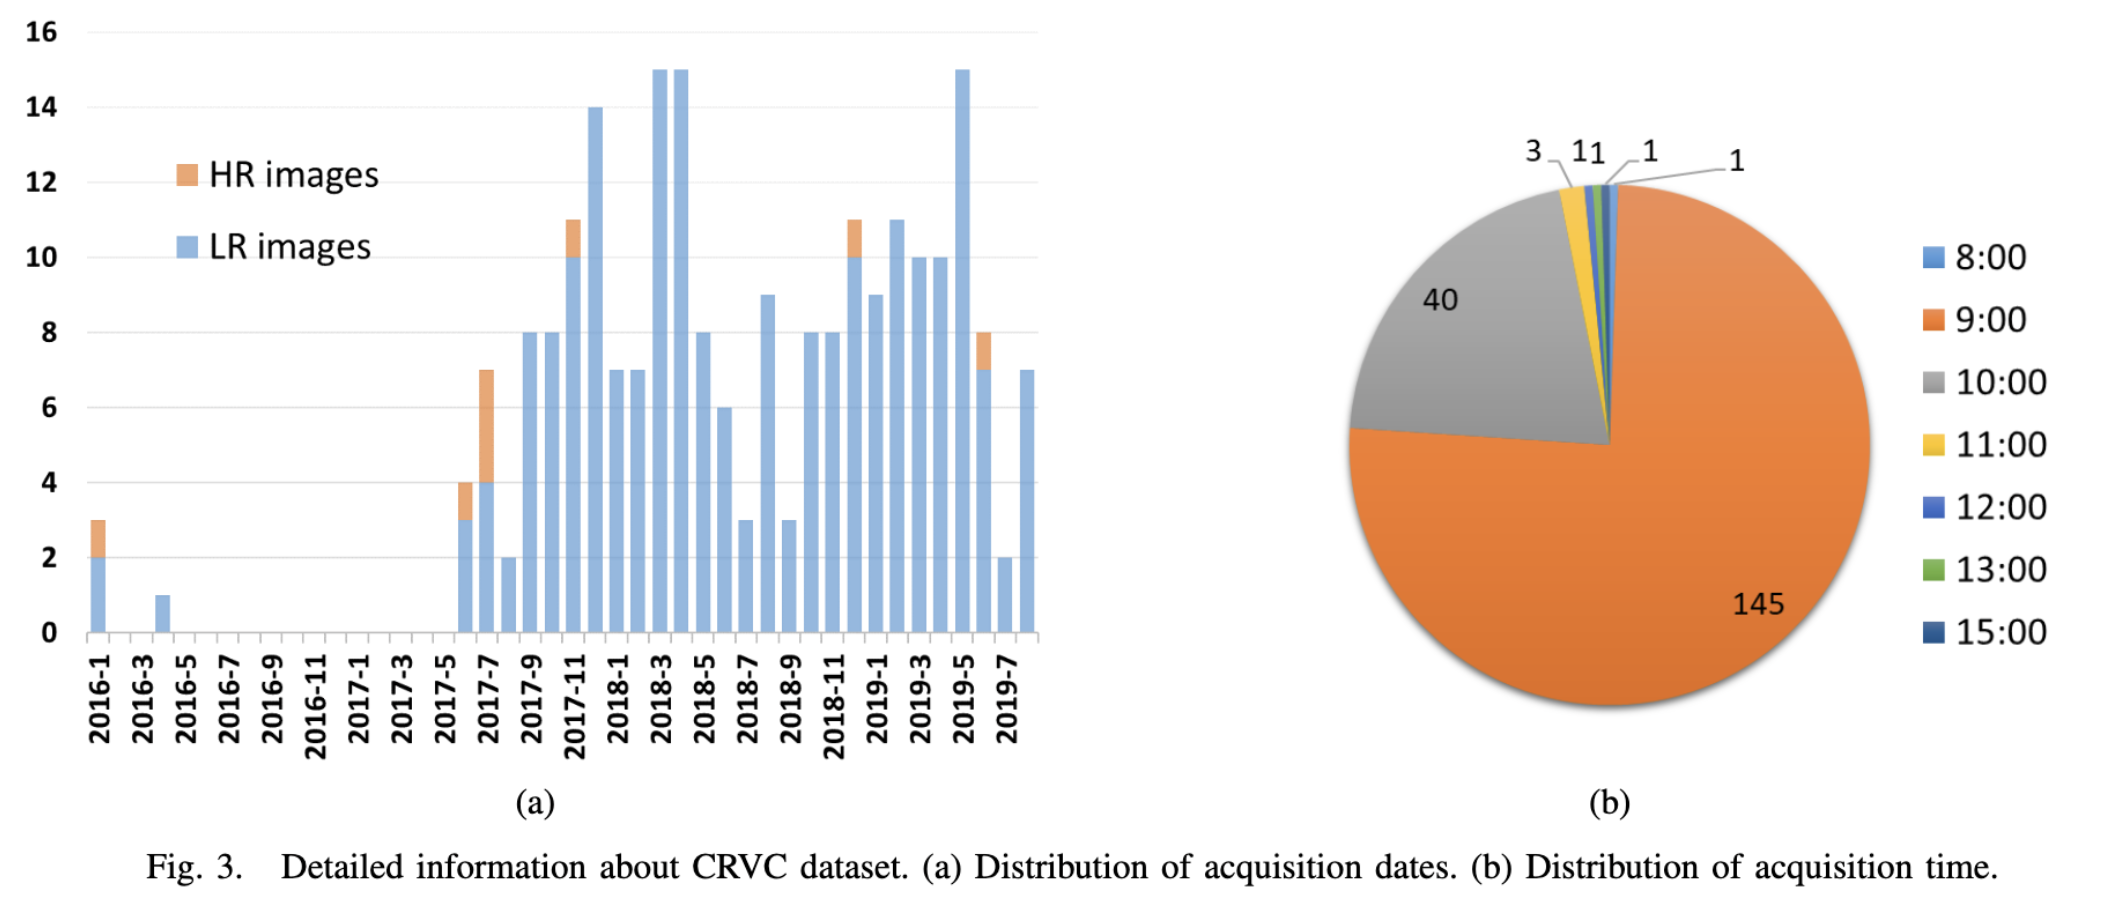
\includegraphics[width=\textwidth]{CRVCtime.png}
    \caption{数据的日期和时间分布}
    \label{fig:CRVCtime}
\end{figure}
\subsection{数据集分析}  
图 ~\ref{fig:CRVCtime} 显示了数据集中LR和HR图像采集的日期和时间分布。可以观察到,数据的分布并不平均,主要集中在2017年5月至2019年7月之间。就8张高分辨率图像的日期而言,它们之间的时间间隔最小为 6 天,最大为 17 个月。 如表格~\ref{tab:date}中数据所示,HR 图像和相应 LR 图像之间的采集时间并不完全一致,平均采集时间差异为 39 分钟。在这种情况下,我们认为短时间内的HR和LR图像中的车辆数目一致。这一假设和实际情况相符并大大降低了建模难度。 
\begin{table}[h]
    \centering
    \caption{HR和LR图像的获取日期与时间}
    \label{tab:date}
    \begin{tabularx}{\textwidth}{CCCC}
      \toprule
      日期 & HR拍摄时间 & LR拍摄时间  \\
      \midrule
      4th January, 2016    & 10:56  &10:36\\
      26th June, 2017      &10:24   & 9:34\\
      2nd July, 2017       &10:20   & 9:36\\
      9rth July, 2017      &10:34   & 9:44\\
      15th July, 2017      &10:30   & 9:41\\
      9th November, 2017   &10:25   & 9:42\\
      19th December, 2018  &10:46   & 9:56\\
      6th June, 2019       &10:35   &10:29\\
      \bottomrule
    \end{tabularx}
\end{table}


\subsection{高分辨率图像处理}  
为了进行计数任务,该数据集在HR图像上标注了车辆的边界及类别。HR图像上标注框的数量作为对应日期的LR图像的真值。标注的边界则作为停车场位置的空间提示信息。该数据集中总共注释了 37852 个车辆实例,包含四类车辆,包括轿车、小型卡车、大型卡车和起重机(图~\ref{fig:vehicle})。不同类别的车辆在尺寸形状上有着很大的不同,分类计数有助于提升计数质量。  各类车辆数量极不平衡,分别为轿车35844辆、小型货车737辆、大型货车1211辆、起重机60辆。 
\begin{figure}[h]
    \centering
    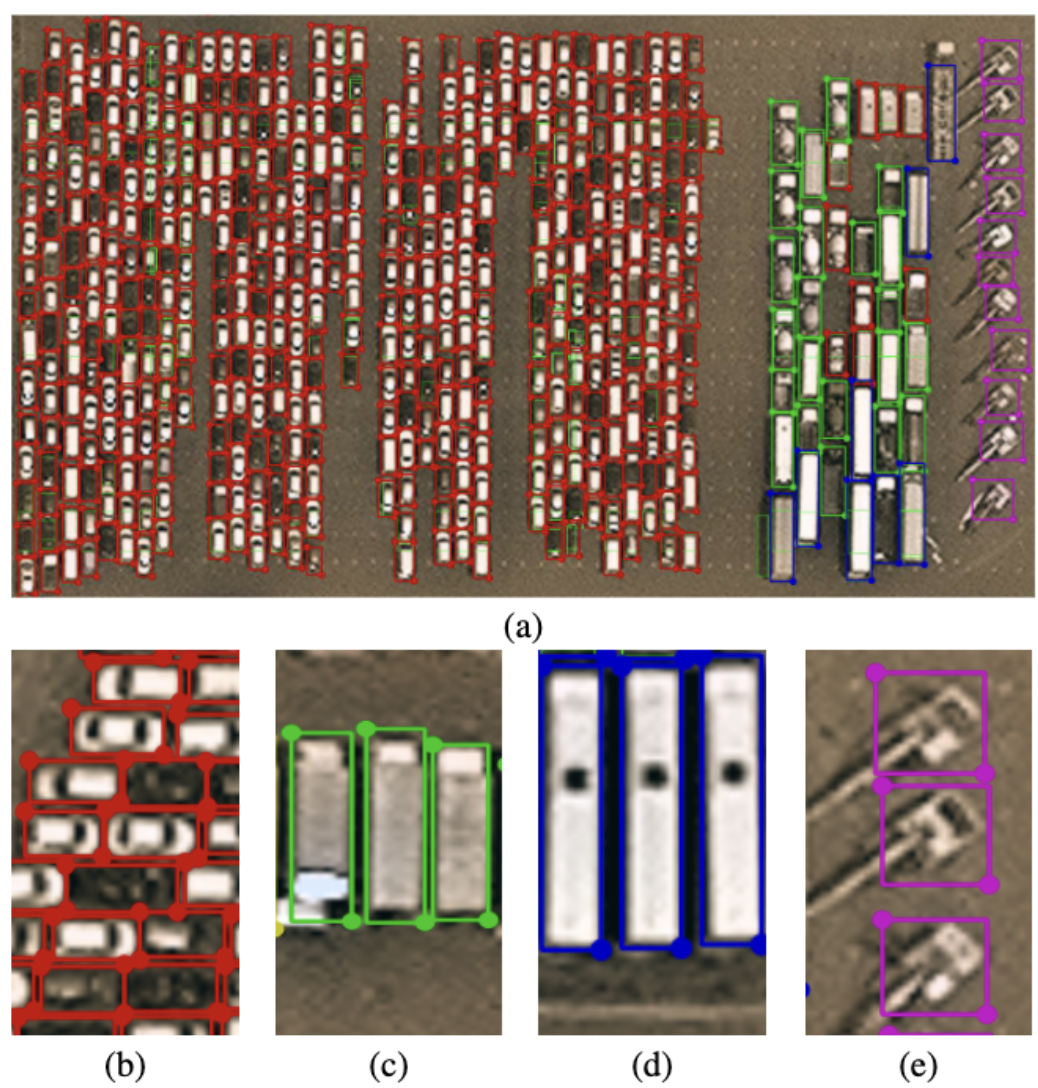
\includegraphics[width=0.5\textwidth]{vehicle.png}
    \caption{HR图像车辆标注及分类}
    \label{fig:vehicle}
\end{figure}

\subsection{低分辨率图像处理}  
数据集中共包含192张低分辨率图像。这些图像在2016至2019年之间被采集,主要分布在2017年6月至2019年8月之间,其中61.5\%的采集间隔在两天以内。如图~\ref{fig:CRVCtime}所示,低分辨率图像的采集时间均为日间,大部分图像拍摄于上午9点到10点。我们可以认为这些图像具有相似的拍摄条件。
不同于高分辨率图像,低分辨率图像的标注要困难的多。因为难以在低分辨率的条件下辨认清晰的车辆轮廓,所以标注车辆覆盖率是一个更可行的方法。由于低分辨率图像的视场较大,车辆区域只占图像中很小的一部分。因此先在HR图像中划出9个区域,在LR图像中的对应位置进行估计(图~\ref{fig:park})。
\begin{figure}[ht]
    \centering
    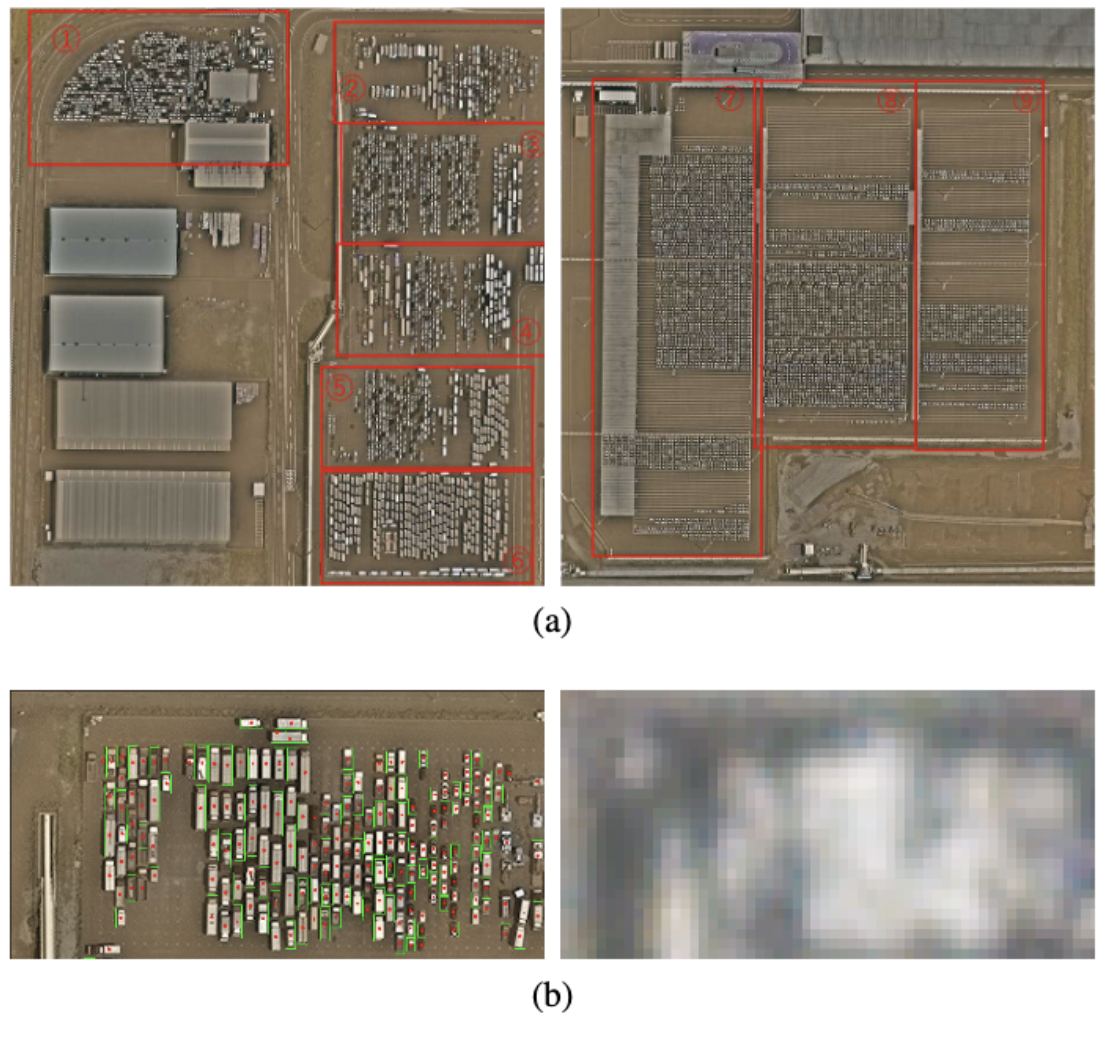
\includegraphics[width=\textwidth]{9park.png}
    \caption{计数区域划分和HR、LR实例图像}
    \label{fig:park}
\end{figure}

低分辨率图像可以分为两类,有对应高分辨率图像的和没有对应高分辨率图像的。对于前者而言,直接从对应高分辨率标注结果中计算覆盖率即可。那些没有HR图像对应的LR图像则由多名专家进行视觉标注并取平均值。
\subsection{空间一致性}  
通过上述对数据集的分析,我们可以看到高分辨率图像和与其对应的低分辨率图像之间间隔时间不大,同时对应的是同一位置。因此我们可以认为在它们上进行的目标计数结果应当也相同。两者所映射的空间信息应该具有一致性,这也给后续处理方法提供了思路。如何应用高分辨率图像信息指导改进低分辨率图像上估计的结果成为提高估计精度的关键节点之一。
\subsection{时间连续性}
单一的低分辨率图像很难得出合理的目标计数估计,然而由于低分辨率遥感图像的短重访周期,我们能得到一段连续的低分辨率图像。比较相邻图像间的变化或者从多个图像间进行学习,可以补充那些单张图像因低分辨率造成的信息缺失。图像间的时间连续性也是指导改进图像计数估计结果的关键因素。
\section{CRVC网络}
CRVC网络是针对CRVC数据集设计的深度学习模型。它以U-Net模型为骨架,设计了跨分辨率空间CRVC数据集中的跨分辨率空间信息和时序信息。通过上述网络估计出密度分布后,使用线性回归模型得出最终目标计数结果。
\subsection{网络设计}
\begin{figure}[h]
    \centering
    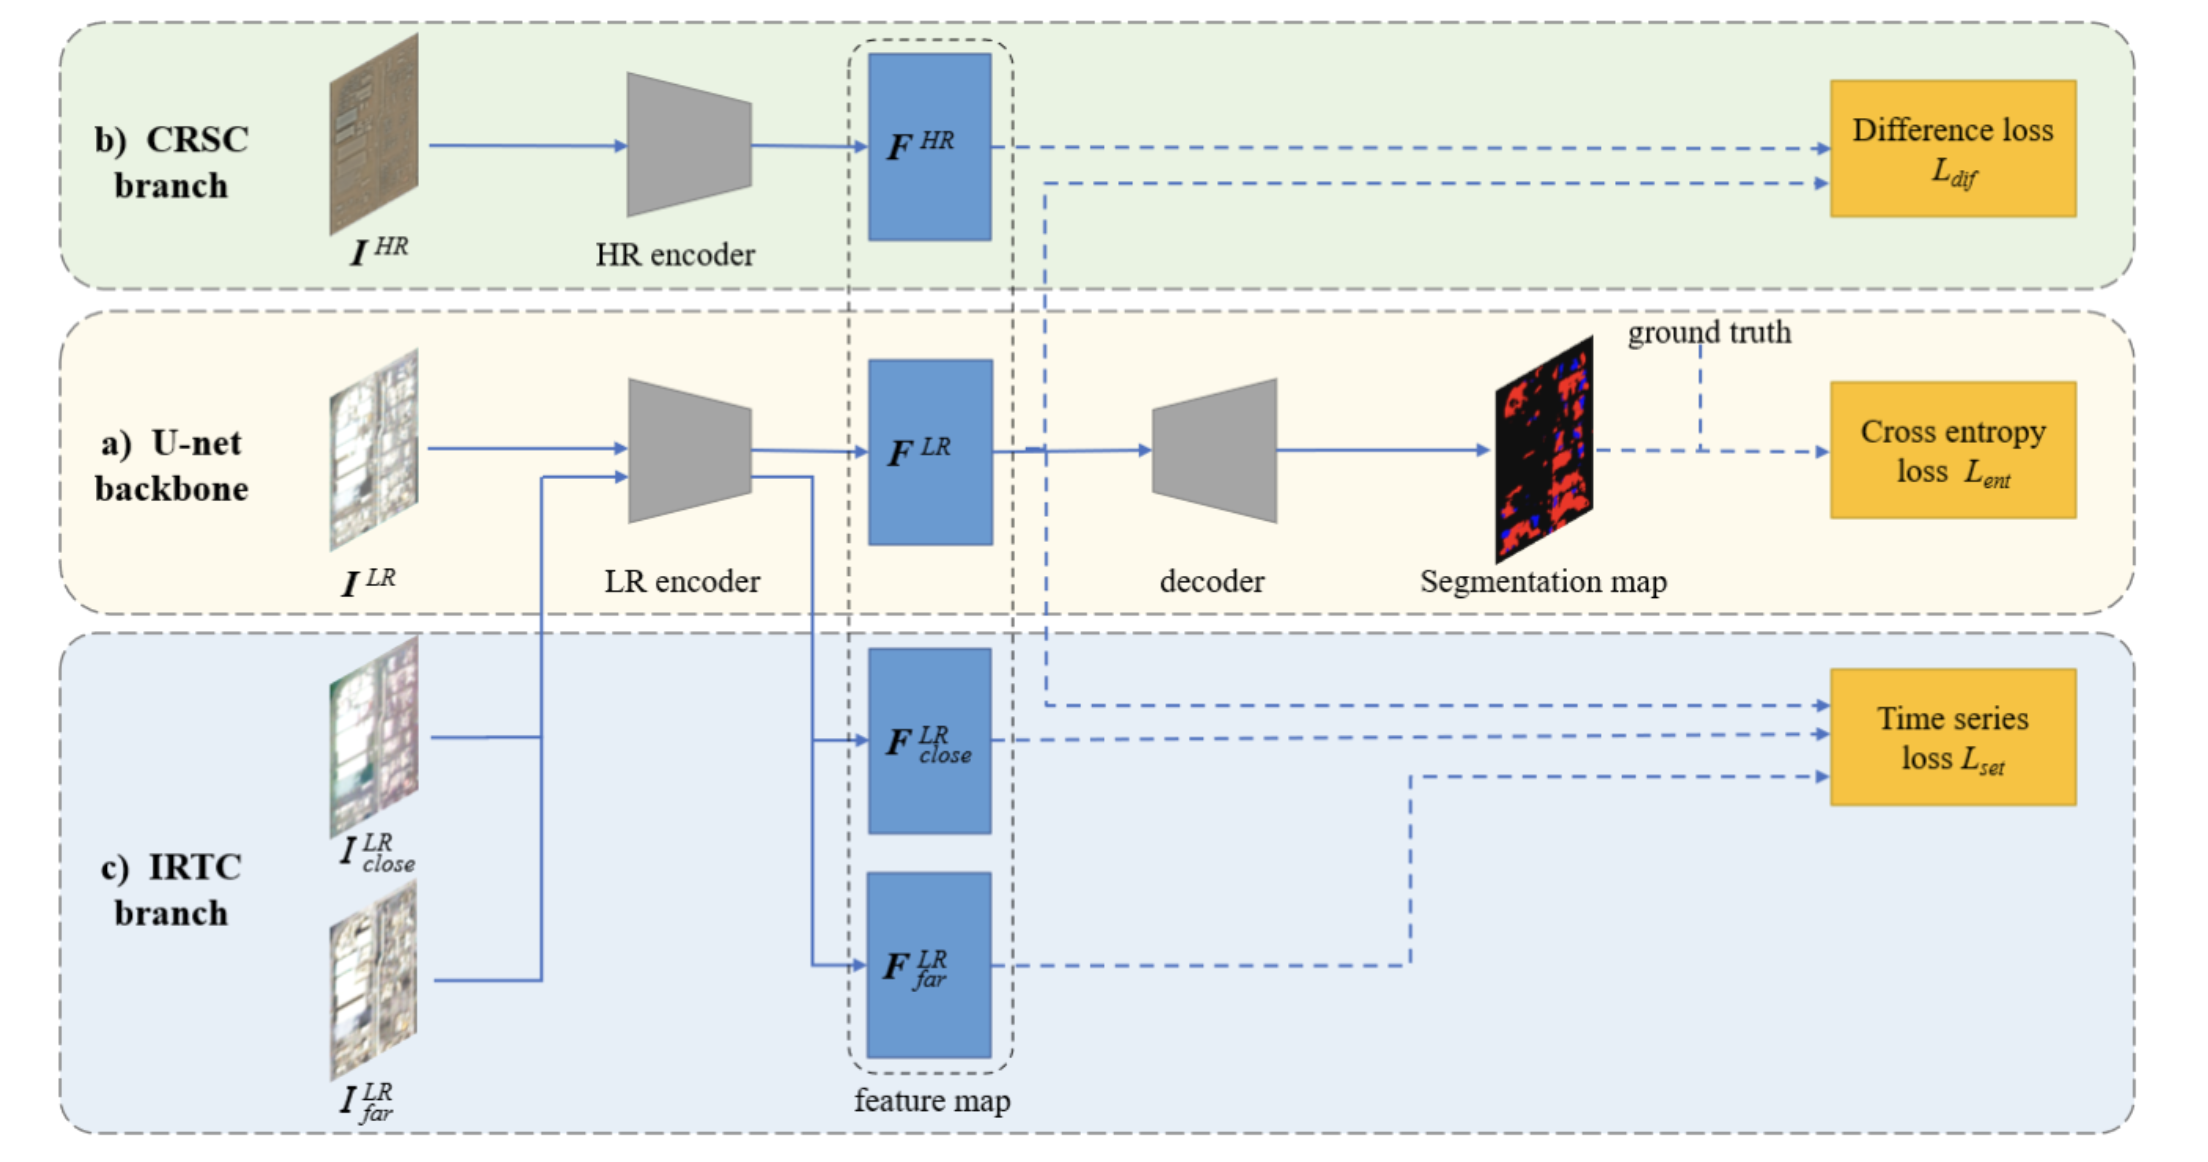
\includegraphics[width=\textwidth]{CRVCnet.png}
    \caption{CRVC网络架构}
    \label{fig:CRVCnet}
\end{figure}

上图~\ref{fig:CRVCnet}展示了模型的基本框架。模型接受4个输入,分别是高分辨率图像输入$I^{HR}$,对应低分辨率图像输入$I^{LR}$,与LR图像时间间隔较近的$I^{LR}_{near}$和与LR图像时间间隔较远的$I^{LR}_{far}$。模型包含两个独立学习的编码器HR encoder和LR encoder,前者用来提取高分辨率图像的特征,后者用来提取3个低分辨率图像的特征。提取出的低分辨率特征和高分辨率特征作差来综合更高精度的信息。之后通过带有跳跃连接的decoder完成分割图的生成。
\subsection{损失函数}
CRVCnet设计了三个损失函数,综合三个损失函数的结果来训练模型。
第一个损失函数为交叉熵损失函数,这个函数常用来衡量概率之间的距离。网络经sigmod输出的分割图也是一种概率分布。用交叉熵衡量其偏差程度有着不错的效果。
\begin{equation}
    \mathcal{L}_{\text {ent }}=-\frac{1}{n} \sum_{i} y_{i} \ln a_{i}
\end{equation}
对于高分辨率和低分辨率图像间的空间一致性,它们之间的差异越小,模型对于真实情况的把握就越好。文章提出了下面的损失函数进行约束。
\begin{equation}
    \mathcal{L}_{\text {dif }}=\sum_{i}\left|F_l^{L R}-F^{HR}_{l}\right|^2
\end{equation}

网络接受3个低分辨图像,分别是有高分辨率对应的低分辨率图像,距离这个低分辨率图像时间较近的图像和距离这个低分辨率图像时间较远的图像。由于时间连续性的约束,日期接近的图像间的差异应该小于日期相隔较远的差异。因此这部分损失函数的设计要求相邻日期图像间的差异更小,日期间隔较远的差异较大。下面的公式同时满足上述条件,且符合最小化损失的要求
\begin{equation}
    \mathcal{L}_{\text {ser }}=\sum_{l=1}^{m} \frac{\left|F_{\text {closel }}^{L R}-F^{L R}{ }_{l}\right|}{\left|F_{\text {far } l}^{L R}-F^{L R}_ l\right|}
\end{equation}
最终的损失函数由各个损失函数加权得到,即
\begin{equation}
    \mathcal{L}=\omega_1\mathcal{L}_{\text {ent }}+\omega_2\mathcal{L}_{\text {dir }}+\omega_3\mathcal{L}_{\text {ser }}
\end{equation}

其中$\omega_1,\omega_2,\omega_3$为各个损失函数的权重,是设定好的超参数。m是特征图的通道数.

\subsection{回归模型}

在CRVC数据集中,车辆在目标区域是密集停放的,而且不存在重叠。因此从分割图上估计出的覆盖率和最终的车辆数目具有线性关系。通过CRVC网络得到的覆盖率分割图,根据低分辨率图像的缩放比例,可以估计出实际面积。通过线性回归,找出参数k来拟合
\begin{equation}
    Number_i=k_i\dots Area_i+b_i
\end{equation}
其中i表示第i类车辆。这些参数通过高分辨率图像的真值计算得到。
